\chapter{Framework Conceptual}
\label{chap2:FC}


\section{Definiciones Básicas}
\label{chap2:Def}

Para empezar este estudio es necesario introducir ciertas nociones y lenguaje que se usarán durante todo el documento. Estos conceptos son usados en la Seguridad y Desarrollo de Software, y son extendibles para lo que se verá en este estudio.

\begin{itemize}
    \item Seguridad - \textit{Security}:
        \\Es una Propiedad que podría tener un sistema, donde asegura la protección de los recursos e información, en contra de ataques maliciosos desde fuentes externas como internas. La Seguridad también involucra controlar que el funcionamiento de un sistema sea como debería ser, y que nada externo o interno genere un error.
    \item Error - \textit{Error}:
        \\Es una acción de caracter humano. Éste se genera cuando se tienen ciertas nociones equivocadas, que causan un Defecto en el Sistema o Código.
    \item Defecto  - \textit{Defect}:
        \\Es una caracterítica que se obtiene a nivel de Diseño, cuando una funcionalidad no hace lo que tiene que realmente hacer. Según la IEEE CSD o \textit{Center for Secure Design} \cite{ieeecsd2}, un defecto puede ser subdividido en 2 partes: falla o \textbf{flaw} y \textbf{bug}, donde la primera tiene que ver con un error de \textbf{alto nivel}, mientras que un bug es un problema de implementación en el Software. Una falla es menos notoria que un bug, dado que ésta es de caracter abstracto, a nivel de diseño del Software.
    \item Falla - \textit{Fail}:
        \\Es un estado en que el Software Implementado no funciona como debería de ser.
    \item Vulnerabilidades - \textit{Vulnerability}:
        \\Es una debilidad inherente del sistema que permite a un atacante poder reducir el nivel de confianza de la información de un sistema. Una vulnerabilidad convina 3 elementos: un defecto en el sistema, un atacante tratando de acceder a ese defecto y la capacidad que tiene el atacante para llevarlo a cabo. Las vulnerabilidades más críticas son documentadas en la \textit{Common Vulnerabilities and Exposures} (CVE) \cite{cve}.
    \item Superficie de Ataque - \textit{Attack Surface}:
        \\Es el conjunto de todas las posibles vulnerabilidades que un sistema puede tener, en un cierto momento, para una cierta versión del sistema, etc.
    \item Amenaza - \textit{Threat}
        \\Es una acción/evento que se aprovecha de las vulnerabilidades del sistema, debilidades, para causar un daño, y que dependiendo del recurso al que afecte el daño puede o no ser reparable.
    \item Ataque - \textit{Attack}
        \\Es el éxito de la amenaza en el aprovechamiento de la vulnerabilidad (explotación de ésta), de tal forma que genera una acción negativa en el sistema y favorable para el atacante.
    \item \textit{Exploit}:
        \\Usar una pieza de software para poder llevar a cabo un ataque sobre un objetivo, intentando \textbf{explotar} la vulnerabilidad de éste. Este tipo de acción permite en consecuencia obtener control en el sistema computacional, en donde la vulnerabilidad permitió su acceso.
    \item Ingeniería Social - \textit{Social Engineering}
        \\El acto de manipular a las personas de manera que realicen acciones o divulguen información confidencial. El termino aplica al acto de engañar con el propósito de juntar información, realizar un fraude, u obtener acceso a un sistema computacional. La definición anterior encontrada en Wikipedia es extendida por el autor del libro ``The Social Engineer's Playbook'' \cite{socEngineeering}, donde agrega que además la Ingeniería Social involucra el hecho de manipular a una persona en realizar acciones que finalmente no son para beneficiar a la víctima. Un ataque de éste tipo también puede llegar a ser realizado tanto \textbf{cara a cara}, como de forma indirecta. Pero el autor del libro indica que siempre hay un \textbf{contacto} previo con la víctima.
    \item Confidencialidad - \textit{Confidentiality} 
        \\Característica o propiedad que debe mantener un sistema para que la información privilegiada de alguna entidad que depende de tal sistema, no sea develada a nadie más que al que le pertenece la información.
    \item Integridad - \textit{Integrity}
        \\Característica o propiedad que asegura que la información no será modificada/alterada nada más que por la entidad a quién le pertenece y con el previo consentimiento de éste.
    \item Disponibilidad - \textit{Availability}
        \\Característica o propiedad que permite que la información esté disponible para quién lo necesite, en el momento que sea. La imposibilidad de obtener data en un cierto instante de tiempo, conlleva a la perdida de esta propiedad.
    \item \textit{Phishing}
        \\Técnica de Ingeniería Social. Mediante el uso de correo elentrónico, links (url's), acortamiento de urls y otras herramientas, se busca que una victima visite un sitio o aprete un link de manera que se de la \textbf{autorización explicita} del usuario para descargar código malicioso o enviar datos a un servidor malicioso. El objetivo de esta técnica es poder obtener información valiosa de la victima o relizar algún daño en el cliente web.
    \item \textit{Malware}
        \\Software creado para realizar acciones maliciosas en la data o sistema de un usuario. Puede ser instalado tanto de forma discreta como indiscreta, siendo la segunda opción causada a través de un ataque previo a cierta vulnerabilidad que permitió la instalación del malware, sin el consentimiento del usuario privilegiado del sistema.
    \item \textit{Man-in-the-Middle}
        \\Ataque que causa una pérdida en la Confidencialidad de la información que es revelada. La causa de este ataque puede ser tanto:
            \begin{itemize}
                \item Por técnicas de Ingeniería Social, entregano un certificado malicioso que el usuario acepta con o sin intención.
                \item A través de vulnerabilidades del sistema que debieron ser explotadas antes para causar el ataque MiTM.
            \end{itemize}
    %\item \textit{Penetration Testing}
    %\item \textit{Fuzzing}
\end{itemize}



% \section{Organizaciones}
% \label{chap2:Orgs}
% Las organizaciones que ,

%     \subsection{OWASP: Open Web Application Security Project}
%     \label{chap2:OWASP}
%     Desde el 2006 la \textit{Open Web Application Security Project} ha estado entregando pautas de cómo desarrollar aplicaciones web, en un ambiente que constantemente está cambiando. Su objetivo principal es buscar y combatir las causas de inseguridad en el desarrollo de Software, proporcionando una gran cantidad de documentación y herramientas aquellos que lo necesiten y no sean expertos en seguridad. Para lograr su cometido, todos los años la OWASP entrega una lista de los Riesgos y Threats más críticos sobre la seguridad de las Aplicaciones Web, de manera de preveer que Desarrolladores de Sistemas o programadores generen vulnerabilidades en el Software que crean.

%     \subsection{IEEE CSD: Center for Secure Design}
%     \label{chap2:IEEECSD}
%     La organización \textit{IEEE Computer Society} lanzó como iniciativa la creación de la \textit{IEEE Cyber Security}, con el objetivo de expandir su participación en el campo de la Ciber Seguridad o \textit{Cyber Security} - u otra forma de llamar al área de la Seguridad Computacional o \textit{Computer Security}. El primer paso realizado para cumplir este objetivo fue iniciar el \textit{IEEE Center for Secure Design} (CSD), que intenta en cambiar el foco en la seguridad desde hayar bugs hasta identificar defectos comunes en Diseño, con la esperanza de que Arquitectos de Software puedan aprender de las equivocaciones de otros \cite{ieeecsd1}.

%     \subsection{W3C: World Wide Web Consortium}
%     Es una comunidad internacional donde organizaciones miembros, trabajadores de tiempo completo y el público, trabajan mano a mano para desarrollar \textit{Web Standards} o Estandares Web. La misión de la W3C es conducir a la \textit{Web} a su máximo potencial, a través del desarrollo de protocolos y guías que aseguran el crecimiento a largo plazo de la \textit{Web}.



\section{Browser}
\label{chap2:Browser}

    \subsection{Arquitectura Cliente/Servidor}
    \label{chap2:ArqCS}
    La web emplea lo que se conoce como una Arquitectura Cliente-Servidor, donde la comunicación entre ambas entidades se basa mediante mensajes de \textit{request-response} o solicitud-respuesta. Con el tiempo la forma en que se comunican estos programas a cambiado, desde iniciar solicitudes de forma secuencial e independiente, hasta solicitar asíncronamente varias peticiones. La evolución que ha tenido el cliente web ha permitido una mejor experiencia para el usuario, pero que conlleva ciertos riesgos que es necesario que el que usa el Browser sea consciente. De la misma manera que podemos afectar a un servidor a través de las solicitudes, las respuestas que el servidor envía al cliente pueden tener consecuencias graves \cite{alcorn2014browser}.


    \subsection{SOP: Same Origin Policy} %listo
    \label{chap2:SOP}

    Es un principio de seguridad implementado (hoy en día) por cada browser existente, su principal objetivo es restringuir las formas de comunicación entre una ventana y un servidor web. \textbf{Same Origin Policy} o \textbf{SOP} es un acuerdo entre varios manufacturadores de navegadores web cómo Microsoft, Apple, Google y Mozilla (entre los más importantes), en donde se definió una estandarización de cómo limitar las funcionalidades del código de scripting ejecutado en el browser del usuario. 

    Este importante concepto nace a partir del Modelo de Seguridad detrás de una Aplicación Web, al mismo tiempo que es el mecanismo más básico que el Browser tiene para protegerse de las amenazas que aparecen en el día a día, haciendo un poco más complicado el trabajo de crear un \textit{exploit}. \textbf{SOP} define lo que es un \textbf{Origen}, compuesto por el \textit{esquema}, el \textit{host/dominio} y \textit{puerto} de la URL. Esta política permite que un Web Browser aisle los distintos recursos obtenidos por las páginas web y que solo permita la ejecución de \textit{Script} que pertenezcan a un mismo \textbf{Origen}. Inicialmente fue definido solo para recursos externos, pero fue extendido para incluir otros tipos de orígenes, esto incluye el acceso local a los archivos con el \textit{scheme} \textbf{file://} o recursos relacionados al Browser con \textbf{chrome://}.

    \textbf{SOP} puede distinguir entre la información que envía y recibe el Web Browser, y solo se aplicará la política a los elementos externos que se soliciten dentro de una página web (recepción de la información). Esta imposibilidad de recibir información de un \textbf{Origen} diferente al del recurso actual, permite disminuir la superficie de ataque (\textit{Attack Surface}) y la posibilidad de explotar alguna vulnerabilidad en el sistema donde reside el Browser. Sin embargo, \textbf{SOP} no pone ninguna restricción sobre la información que el usuario puede enviar hacia otros. 

    \textbf{SOP} es la base de la mayoría de los principios de seguridad, dado que sin él cualquier sitio podría accesar a la información confidencial de un usuario o de cualquier otro sitio. Por tanto es sencillo entender la razón de la existencia de SOP, se desea proteger la información del usuario, sus cookies, token de autenticación, etc. de las amenazas existentes en la Internet.


    %referencia de chrome Zalewsk08
    En \cite{Zalewsk08} menciona que no existe una sola forma de SOP, si no que es una serie de mecanismos que superficialmente se parecen, pero al mismo tiempo poseen diferencias:

    \begin{itemize}
        \item SOP para acceso al DOM: se dará permiso de modificar el DOM solamente aquellos scripts que ponean el mismo dominio, puerto (para todos los browsers excepto Internet Explorer) y protocolo.
        \item SOP para el objeto XMLHTTPRequest
        \item SOP para \textit{cookies}
        \item SOP para Flash, donde usa políticas para realizar peticiones fuera del dominio através de un archivo \textbf{crossdomain.xml}
        \item SOP para Java
        \item SOP para Silverlight, parecido al de Flash solo qe utiliza otros elementos.
    \end{itemize}

        
   Tanto para los atacantes como desarrolladores de Software, SOP puede llegar a ser bastante molesto. Para el primero, la respuesta es obvia, pero para el segundo está el problema de ¿cómo poder aislar los componentes no confiables o parcialmente confiables, mientras que al mismo tiempo se pueda tener una comunicación entre ellos de forma segura? Ejemplo de esto son los Mashup \cite{barth2009securing}, que permiten juntar contenido de terceros en una misma página por medio de frames, etc. 
        
    Existen excepciones que permiten evitar el uso de SOP, pero como es de esperar esta vía puede ser mal usada por los atacantes en contra del usuario y de la Aplicación Web. Dentro de las excepciones están los elementos en HTML \(<\) script \(>\), \(<\)img\(>\), \(<\)iframe\(>\) y otros, que si bien permiten la comunicación entre diferentes orígenes, un mal uso de este puede causar grandes estragos, desde la eliminación de registros en una base de datos hasta la propagación de un gusano o virus.
        
    Queda decir que si bien SOP entrega una capa de seguridad al usuario y a la Aplicación Web, contra cierto tipo de ataques (muchas veces del tipo de ataques de principiantes), esto no es suficiente. Es responsabilidad del desarrollador de Software poseer las herramientas necesarias para asegurar la confidencialidad e integridad del sistema a través de otros métodos de seguridad.
    

    %Ver libro de Browser hacker handbook

    \subsection{Markup Languages}
    \label{chap2:markup}
        Un lenguaje de marcado sigue tradicionalmente un \textit{Standard Generalized Markup Language}, de manera que entrega una semántica apropiada para representar o mostrar contenido, placeholders de aplicaciones y datos. Cada página mostrada por el navegador, sigue las instrucciones que el lenguaje de marcado le da al browser para mostrar el contenido. HTML y XML son los más conocidos en el mercado. Ambos lenguajes tienen sus especificaciones en la W3C o World Wide Web Consortium.

        \subsubsection{HTML: HyperText Markup Language}
        \label{chap2:HTML}
        HTML \cite{htmlSpec} es conocido por ser un \textit{Simple Markup Language} o lenguage de marcado simple, usado principalmente para crear documentos de hypertextos que son posibles de portar desde una plataforma a otra, sin problemas de compatibilidad. Un documento HTML consiste de un árbol de elementos y texto, cada uno de esos elementos es denotado por un tag inicial y uno final; estos tags pueden ir aninados y la idea es no se superponen entre ellos. Un HTML User Agent o Browser consume el HTML y lo parsea para crear un árbol DOM, que es la representación en memoria del documento HTML.
        Una característica importante de este lenguaje de marcado es su flexibilidad ante los errores, esto es que en alguna ocasiones el programador perfectamente podría sobrarle un signo y HTML no le daría mayor importancia mientras no afecte a la estructura global de la página. Normalmente esta característica aprovechada por los atacantes para insertar'cósigo scripting en las páginas.
        %Para poder crear una Aplicación interactiva y segura con HTML, es necesario evadir la creación de vulnerabilidades por donde los atacantes podrían comprometer la integridad del sitio o del usuario que descarga el recurso HTML del sitio atacado. Típicos errores que deben ser evitados cuando se usa scripting con HTML, es que los scripts en HTML tienen una semántica run to completion, esto quiere decir que el browser ejecutará el script mucho antes de que se realice el parsing del documento o gatillar un evento; este tipo de comportamiento es el que los atacantes aprovechan para realizar sus ataques.


        \subsubsection{XML: eXtensible Markup Language}
        \label{chap2:XML}
        Este lenguaje de marcado tiene una estrecha relación con HTML, pero a diferencia de este último tiene una sintáxis y semántica más rígida ya que sigue al pie de la letra un lenguaje libre de contexto. Este tipo de lenguaje es ideal para el transporte de data entre \textit{web Services} o interacciones \textbf{RPC}, dado que no hay forma de como malinterpretar la data.


    \subsection{CSS: Cascading Style Sheets}
    \label{chap2:css}
    Es un lenguaje usado es usado junto a HTML o XML para definir la capa de presentación de las páginas web que el navegar renderiza al usuario. La W3C o World Wide Web Consortium se encarga de la especificación de las hojas de estilos para que los browser sean capaces de interpretar bajo estándares y aseguren ciertos niveles de calidad. Una hoja de estilo se compone de una lista de reglas. Cada regla o conjunto de reglas consiste en uno o más selectores y un bloque de declaración, más los estilos a aplicar para los elementos del documento que cumplan con el selector que les precede. 


    \subsection{DOM: Document Object Model}
    \label{chap2:DOM}
    Es una \textit{API} independiente del lenguage y multiplataforma para HTML válido y bien formado, que define la estructura lógica de un documento que permite ser accedido y manipulado. DOM es una especificación que permitiría a programas JavaScript modificar la estructura del contenido de una página y además de ser portable para los Browser, en el tiempo en que se usaba Dynamic HTML para esa tarea. Posteriormente la \textit{W3C} \cite{w3c} formó el \textit{DOM Working Group} y con ello se creó la especificación a través de la colaboración de muchas empresas y expertos. La arquitectura de esta \textit{API} se presenta en la Figura \ref{fig:DOM}, donde el \textit{Core Module} es donde están las interfaces que deben ser implementadas por todas las implementaciones conformes de DOM. Una implementación de DOM puede ser construida por uno o más módulos dependiendo del host, ejemplo de esto: la implementación de DOM en un servidor, donde no es necesaria la implementación de los módulos que manejen los triggers de eventos del mouse.
            
    \begin{figure}[h]
        \centering
        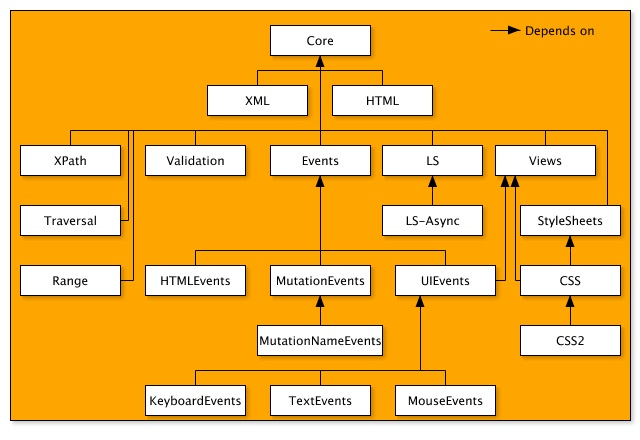
\includegraphics[width=0.65\textwidth]{figures/dom-architecture.jpg}
        \caption{Arquitectura de DOM \cite{w3c}}
        \label{fig:DOM}
    \end{figure}
            
    La interfaz de \textit{DOM} fue definida por el OMG IDL y fue construida para ser usada en una gran variedad de ambientes y aplicaciones. El documento parseado por DOM se transforma en un gran objeto, tal modelo captura la estructura del documento y el comportamiento de éste, además de otros objetos de lo que puede estar compuesto y las relaciones entre ellos. Cada uno de los nodos representa un elemento parseado del documento, el cuál posee una cierta funcionalidad e identidad. La estructura de árbol del DOM construido puede llegar a ser gigantezca, puede llegar a almacenar más de un árbol por cada documento que parsea. 
            
    \subsection{Javascript, VBScript y otros}
    \label{chap2:JS}
    Ambos son lenguajes de scripting orientados a objetos. Javascript fue desarrollado por Netscape mientras que VBScript fue desarrollado por Microsft para Internet Explorer, los dos siguen el estandar del lenguage de scripting \textbf{ECMAScript}. Dado que VBScript no era usado por muchos y no tenía soporte para otros navegadores más que Internet Explorer, Microsft decidió abandonarlo.

    Muchos piensan que JavaScript es un lenguage interpretado, pero es más que eso. Javascript es un lenguage de \textbf{scripting dinámico} (por tanto no es tipificado) que soporta la construcción de objetos basados en \textbf{prototipos}. Esto quiere decir que a diferencia de un lenguage de programación orientado a objetos como Java, un lenguage orientado a prototipos no hace la distinción entre clases y objetos (clase instanciada), son simplemente objetos. Y cómo tal al ser construido con sus propidades iniciales, es posible poder agregar o remover propiedades y métodos de forma dinámica (durante el runtime) tanto a un objeto como a la clase.
            
    Javascript puede funcionar tanto como un lenguage de programación procedural o como uno orientado a objetos. Firefox usa una implementación en C de Javascript llamada \textit{Spider Monkey}, Google Chrome/Chromium tiene un motor de JavaScript llamado \textit{V8} e Internet Explore no usa realmente JavaScript si no que \textit{JScript} (hace lo mismo que las otras implementaciones solo que difiere en el sistema operativo que utiliza) que en este caso se llama \textit{Chakra}.
            
    Si bien es posible comprender que JavaScript posee increíbles posibilidades para la creación de \textit{RIA} (Rich Internet Applications), en \cite{barth2009attacks} se muestra que puede llegar a ser un fracaso si es que no se toman en cuenta ciertas vulnerabilidades inherentes al lenguage. Estas vulnerabilidades que pueden llegar a ser criticas, a menudo permiten a un comunicante comprometer completamente a la otra parte. La misma naturaleza de JavaScript que permite la modificación en runtime de los objetos, puede llegar a ser aprovechada de esta situación; en la cita toma por ejemplo la comunicación entre los elementos de un \textit{Mashup}.


    \subsection{CORS: Cross-Origin Resource Sharing}
    \label{chap2:CORS}
    Cómo lo define su nombre es un mecanismo que permite al cliente realizar request entre sitios de diverso \textit{Origen}. \textit{CORS} define una forma en que el Browser y el Servidor Web puedan interactuar para determinar si permitir o no el request a otro origen. Un Browser utiliza SOP para restringuir los request de la red y prevenir al cliente de una Aplicación Web ejecutar código que se encuentra en un origen distinto, además de limitar los request HTTP no seguros que podrían tratar de generar un daño. CORS extiende el modelo que el Browser maneja e incluye:
        
        \begin{itemize}
            \item Un header en la respuesta/response del servidor solicitado llamado \textit{Access-Control-Allow-Origin}, donde se debe escribir el origen que tendrá acceso a los recursos solicitados al servidor. Si el valor de la respuesta del servidor coincide con el \textit{origen} de quién lo solicitó, se podrá realizar el uso del recurso en el navegador, de lo contrario se generará un error.
            \item Otro header llamado \textit{Origin} pero esta vez en el request de la solicitud, para permitir al Servidor hacer cumplir las limitaciones en las peticiones de distinto origen.
        \end{itemize}
        Existen ciertos métodos en HTTP que necesitan realizar un \textit{pre-vuelo} antes de ser ejecutados, si la response del servidor es afirmativa luego se enviará el request original con el método que se debió confirmar su utilización. Para el caso de los métodos GET y POST, los más usados, este pre-vuelo no es necesario y se puede enviar el request inmediatamente.
        
        La gran diferencia de CORS con cualquier otro método de que permita hacer request hacia un origen distinto, es que el Browser por default no enviará ningún tipo de información que permita identificar al user. De esta manera se puede disminuir considerablemente las amenazas en la confidencialidad, pues el atacante no podrá hacerse pasar por un usuario del que no tiene información.
        
        Casi todos los navegadores web, a diferencia de Internet Explore \cite{bookWebAppSec}, realizan sus solicitudes a servidores de  diverso origen por medio de la interfaz \textit{XMLHTTPRequest}, en el caso de Internet Explorer esta se llama \textit{XDomainRequest}.

    \subsection{HTTP: Hypertext Transfer Protocol}
    \label{chap2:HTTP}
    El Protocolo de la capa de Aplicación conocido como HTTP fue creado en los años 90 por el W3C o \textbf{World Wide Web Consortium} y la \textbf{Internet Engineering Task Force}, define una sintaxis y semántica que utilizarían los software basados en una arquitectura Web para comunicarse. El protocolo sigue un esquema de pregunta-respuesta o \textit{request-response}, donde un cliente solicita un recurso que el servidor posee, y el servidor entrega una respuesta de acuerdo al recurso solicitado. La forma en que se localiza un recurso es mediante la dirección URL o \textit{Uniform Resource Locator}

        \subsubsection{HTTP Headers}
        \label{chap2:headers}
        HTTP es la implementación de la capa de aplicacón del modelo OSI que sigue todo dispositivo que desea conectarse a la Internet. Los headers o cabeceras que utiliza este protocolo permiten configurar la comunicación entre un \textit{Web Server} y un cliente web, en este caso con el Browser. Estos headers indican \textbf{dónde} debe ir el mensaje y \textbf{cómo} deben ser manejados los contenidos del mensaje. En cada petición o \textit{request} del Navegador, éste debe especificarlos para que el servidor pueda enteder las peticiones; de la misma manera, el servidor enviará cabeceras que el cliente también debe entender. Algunos \textit{headers} son necesarios y hasta obligatorios, para algunos servidores, y en otros da lo mismo como vayan.


        \subsubsection{Canales de comunicación en HTTP}
        \label{chap2:comunHTTP}
        \begin{enumerate}
            \item postMessage

            \item XHR: XMLHttpRequest

            \item WebSockets
        \end{enumerate}


%%%%%%%%%%%%%%%%%%%%%%%%%%%%%%%%%%%%

\section{Desarrollo de Software Seguro y Diseño de Software Seguro}
\label{chap2:SSD}

La filosofía detrás de \textit{Secure Software Developmet} es que detrás de cada etapa de desarrollo del software, se tengan en cuenta que los prinicipios de Seguridad: Confidencialidad, Integridad, Disponibilidad, Auditoría. Para cumplir este cometido es que se deben llegar a políticas y reglas que aseguren la Seguridad como una propiedad sistémica.

Varias comunidades tienen diferentes enfoques y técnicas de cómo asegurar la Seguridad en los sistemas, muchas pueden incluso tener similitudes y hasta trabajar juntas. En este trabajo, el enfoque tomado es aquél que busca entregar la propiedad de seguridad a través del entendimiento de un sistema a un alto nivel, identificando las amenazas durante la elicitación de requerimientos, de manera que se pueda extraer las posibles amenazas que podrían existir y utilizando elementos de diseño para hacer cumplir los principios de seguridad necesarios por el sistema; este enfoque es el que se dedica la comunidad de \textit{Secure Software Design}. 


Fernandez \cite{fernandez2013security} sostiene que para construir un sistema seguro es necesario realizarlo de manera sistemática de tal manera que la seguridad sea parte del integral de cada una de las etapas del Desarrollo de Software - de inicio a fin. El enfoque que propone es ingenieril y por tanto es aplicable incluso para sistemas \textit{legacy}, donde es posible hacer ingeniería inversa para comprobar si existen o no los requerimiento de seguridad implementados, de manera que permite generar un estudio con la intención de comparar y mejorar nuevos sistemas. En su libro \cite{fernandez2013security} presenta una completa metodología para construir sistemas seguros a partir de patrones de diseño, a los cuales nombra como \textbf{Security Patterns}.

Como parte de la metodología propuesta, se plantea que para diseñar primero se deben entender las posibles amenazas a las que está expuesto el sistema. La identificación de Amenazas [Bra08a] [Fer06c] es la primera tarea que presenta la metodología, que considera las actividades en cada caso de uso del sistema.


\section{Arquitectura de Referencia o Reference Architecture (RA)}
\label{chap2:ArqRef}
%usar \cite{Avgeriou2003}

Una arquitectura de Referencia, de acuerdo a la \textit{Open Security Architecture} o OSA\cite{openSecArch}, es considerado un elemento que describe un \textbf{estado de ser} y debe representar aceptadas buenas practicas. En \cite{Avgeriou2003} se explica que una RA es una arquitectura de software genérica y estandarizada, para un dominio particular e independiente de la plataforma o detalles de implementación. Lo que debe incluir son los componentes principales y fundamentales del sistema, más la interacción entre éstas unidades. Una RA es una herramienta que permite facilitar el entendimiento de sistemas complejos y su apropiada construcción a sistemas reales. Si bien una RA es usada principalmente para capturar los \textit{concerns} de los \textit{Stakeholders} al comienzo de un Desarrollo de Software, también puede ser usada para educar al realizar la unión de ideas y terminologías usadas por diversos sistemas que se asemejen, sin tener que preocuparme de los detalles de implementación.


\section{Patrones}
\label{chap2:Patt}

\section{Patrones de Seguridad}
\label{chap2:SecPatt}

\section{Patrones de Mal Uso}
Para diseñar sistemas seguros, se es necesario identificar las posibles amenazas que un sistema puede sufrir. Papers como \cite{fernandez2013security, fernandez2006defining, fernandez2007attack, braz2008eliciting} describen el desarrollo de una metodología completa para encontrar amenazas, a través del análisis de actividaddes de los casos de uso del sistema buscando como podría un atacante interno o externo socavar las bases de esas actividades. Es importante no confundir \textit{Attack Patterns} con \textit{Misuse Pattern}, pués claramente en \cite{ModMisusePatt, fernandez2013security} dejan explícito que un \textit{Attack Patttern} es una acción que lleva a un mal uso o \textit{misuse}, o acciones \textbf{específicas} que toman ventaja de las vulnerabilidades de un sistema, como por ejemplo un \textit{buffer overflow}. A partir de los trabajos \cite{fernandez2007attack, yoshioka2006development, yoshioka2007integration}  se hace la unión de los conceptos de \textit{Attack Patttern} para dar forma a la definición de \textit{Misuse Pattern} \cite{ModMisusePatt, pelaez2009misuse, fernandez2010worm, hashizume2011misuse, munoz2011misuse, fernandez2012misuse, alkazimi2014, encinamisuse}. Esta nueva definición indica entonces indica que:
\begin{center}
    Un patrón de mal uso o \textit{Misuse Pattern} describe, desde el punto de vista del atacante, qué tipo de ataque es realizadom ()
\end{center}
The misuse pattern describes, from the point of view of the attacker, how a type of at-
tack is performed (what units it uses and how), analyzes ways of stopping the attack by
enumerating possible security patterns that can be applied for this purpose, and describes
how to trace the attack once it has happened by appropriate collection and observation
of forensic data. It also describes precisely the context in which the attack may occur



Sin embargo, cuando un sistema ya está diseña y construido, como es el caso del Web Browser, lo que va a importar es saber \textbf{cómo} los componentes del sistema, pueden ser usados por el atacante para alcanzar sus objetivos. Un \textit{Misuse Pattern} o \textbf{Patrón de Mal Uso} describe, desde el punto de vista del atacante, cómo un tipo de ataque es realizado, indicando \textbf{qué} componentes usa y \textbf{cómo}. Además analiza las formas de detener el ataque a través de un listado de posibles \textit{Security Patterns} o \textbf{Patrones de Seguridad} que pueden ser aplicados para esa situación, y describe cómo poder seguir el rastro de un ataque una vez que ha sido realizado con éxito en el sistema, a través de data forense. Además describe un contexto en dónde puede ocurrir el ataque.

